% title: A bounded loop carries state between iterations
% description: The condition and iteration limit determine whether to run the body. The body returns the next state, and termination returns the final state.
\documentclass[tikz,border=5pt]{standalone}
\usetikzlibrary{arrows.meta,calc,shapes.geometric}
\definecolor{numeric}{HTML}{4477AA}
\definecolor{textual}{HTML}{AA4499}

\tikzset{
    box/.style={draw, line width=0.8pt, minimum height=0.8cm,
                minimum width=1.8cm, inner sep=6pt, align=center},
    ir/.style={box},
    flow/.style={-{Stealth[length=5pt]}, line width=0.9pt},
    feedback/.style={flow, dashed},
    note/.style={font=\small, align=center},
    choice/.style={diamond, draw, line width=0.8pt,
                   aspect=2, inner sep=2pt, align=center},
}

\newcommand{\irframe}[2]{
    \draw[line width=0.8pt] #1 rectangle #2;
}

\newcommand{\transformarrow}[4][above]{
    \draw[flow] (#2) -- node[#1=6pt,note] {#4} (#3);
}

\begin{document}
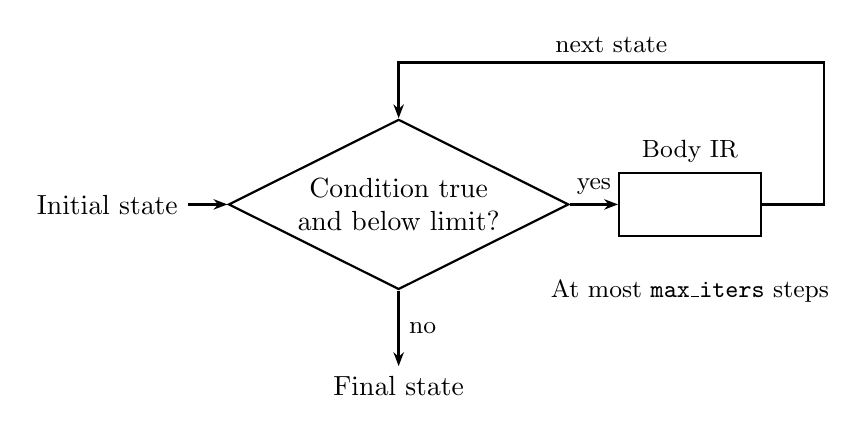
\begin{tikzpicture}

    \node[align=center] (state) at (0,0) {Initial state};
    \node[choice] (cond) at (3.7,0) {Condition true\\and below limit?};
    \node[ir, label={[note]above:Body IR}] (body) at (7.4,0) {};
    \node[align=center] (final) at (3.7,-2.3) {Final state};
    \draw[flow] (state) -- (cond);
    \draw[flow] (cond) -- node[above,note] {yes} (body);
    \draw[flow] (cond) -- node[right,note] {no} (final);
    \draw[flow] (body.east) -- (9.1,0) -- (9.1,1.8)
        -- node[above,note] {next state} (3.7,1.8) -- (cond.north);
    \node[note] at (7.4,-1.1) {At most \texttt{max\_iters} steps};

\end{tikzpicture}
\end{document}
